\documentclass[10pt]{beamer}
\usepackage[slovak]{babel}
\usepackage[utf8]{inputenc}
\usepackage{graphics}
\graphicspath{{img/}}
\usepackage{listings}
\usepackage{hyperref}
\usetheme{Berlin}
\usecolortheme{orchid}
\setbeamertemplate{footline}[frame number]

\title{Typografie a publikování - 5.projekt}
\subtitle{Dátové štruktúry - Binárny strom}
\author{Adrián Bobola}
\institute{Vysoké učení technické v~Brně\\
Fakulta informačních technologií}
\date{\today}

%strana 1
\begin{document}
\begin{frame}
    \titlepage
\end{frame}

%strana 2
\begin{frame}{Obsah prezentácie}
    \tableofcontents
\end{frame}

%strana 3
\section{Úvod do dátových štruktúr}
\begin{frame}{Typy dátových štruktúr}
    Dátové štruktúry umožňujú ukladanie dát do rôznych typov usporiadaní.
    Medzi najznámejšie dátové štruktúry patrí: 
    \begin{itemize}
        \item{Pole (array)}
        \item{Zoznam (list)}
        \item{Zásobník (stack)}
        \item{Strom (tree)}
        \item{Hašovacia tabuľka (hash table)}
    \end{itemize}
    Dnes sa bližšie pozrieme na dátovú štruktúru binárneho vyhľadávacieho stromu.
\end{frame}

%strana 4
\section{Binárny strom}
\begin{frame}{Binárny vyhľadávací strom}
    \begin{itemize}
        \item{Jedná sa o~dátovú štruktúru založenú na binárnom strome.}
        \item{Skladá sa z~koreňa stromu, vnútorných uzlov a listov.}
        \item{Prvky sú usporiadané tak, aby v~strome bolo možné rýchlo vyhľadať požadovanú hodnotu.}
        \item{To zabezpečujú nasledujúce vlastnosti:}
            \begin{itemize}
            \item{Každý uzol má najviac dvoch potomkov (ľavý + pravý)}
            \item{Každému uzlu je priradený určitý kľúč, podľa ktorých sú uzly usporiadané}
            \item{Ľavý podstrom obsahuje iba kľúče menšie ako je kľúč tohto uzlu}
            \item{Pravý podstrom obsahuje iba kľúče väčšie ako je kľúč tohto uzlu}
            \end{itemize}
    \end{itemize}
\end{frame}

%strana 5
\begin{frame}{Binárny vyhľadávací strom}
    \begin{center}
    \begin{figure}
        \scalebox{0.60}{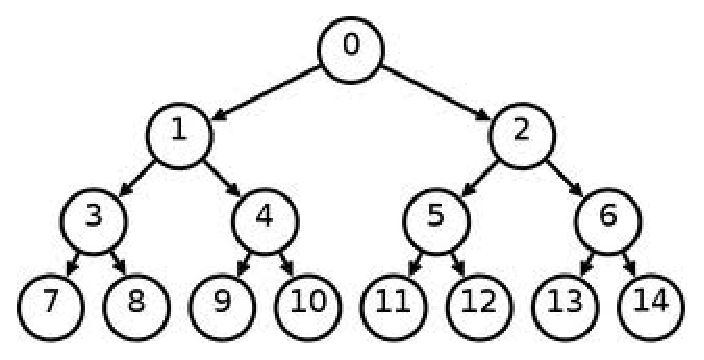
\includegraphics{binary_tree.eps}}
        \caption{Binárny vyhľadávací strom}
    \end{figure}
    \end{center}
\end{frame}

%strana 6
\section{Operácie nad BVS}
\begin{frame}{Operácie nad BVS}
    \begin{itemize}
        \item{\emph{Vkladanie uzlu:}}
        \begin{itemize}
            \item{Vložený uzol je potrebné naviazať na jeho otca a prípadne na vkladaný uzol správne
            naviazať jeho synov.}
            \end{itemize}
        \item{\emph{Odstránenie uzlu:}}
            \begin{itemize}
            \item{Uzol bez synov - korekcia ukazateľa v~uzle otca.}
            \item{Uzol s~jedným synom - korekcia ukazateľa v~uzle otca.}
            \item{Uzol s~dvoma synmi - nahradenie uzlu s~\uv{najhlbším} uzlom v~strome a následné odstránenie tohto uzla.}
            \end{itemize}
        \item{\emph{Prechody stromom:}}
            \begin{itemize}
            \item{Do šírky (level-order)}
            \item{Do hĺbky (pre-order, in-order, post-order)}
            \end{itemize}
        \item{\emph{Ďalšie operácie podľa typu stromu:}}
            \begin{itemize}
            \item{Init, Insert, Search, Copy, Delete a pod.}
            \end{itemize}
    \end{itemize}
\end{frame}

%strana 7
\begin{frame}{Operácie nad BVS - vkladanie}
    \begin{center}
    \begin{figure}
        \scalebox{0.15}{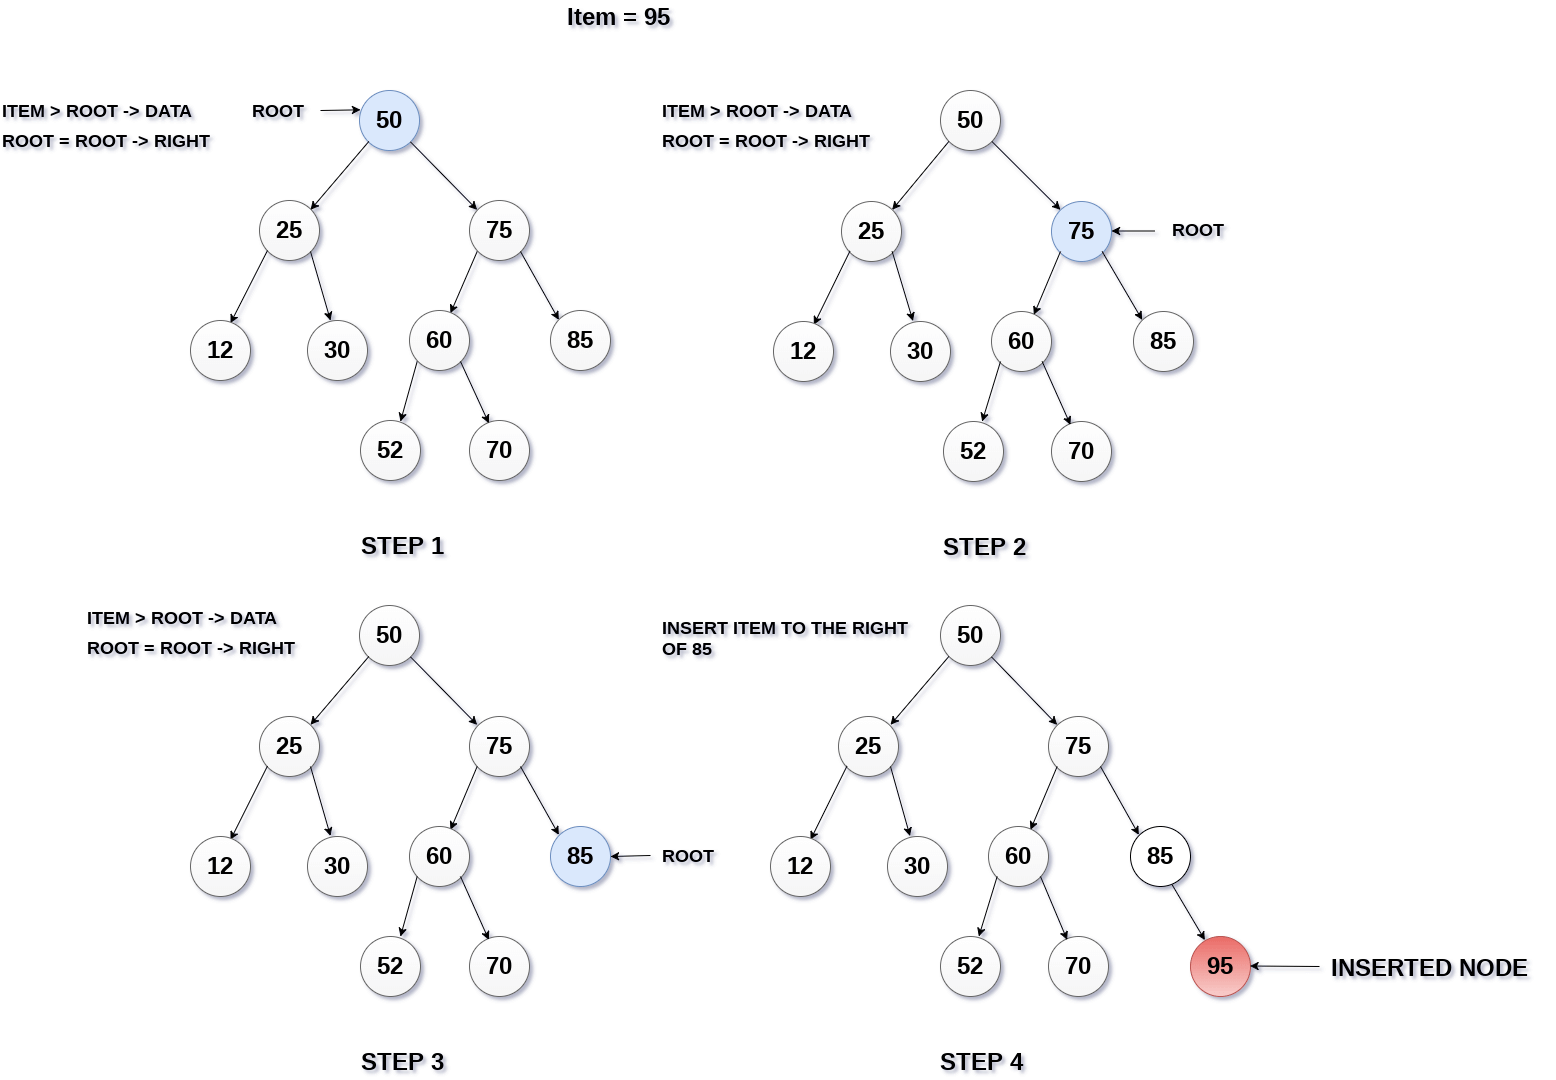
\includegraphics{binary_tree_insert.png}}
        \caption{Binárny vyhľadávací strom - vkladanie nového uzlu}
    \end{figure}
    \end{center}
\end{frame}

%strana 8
\begin{frame}{Operácie nad BVS - mazanie}
    \begin{center}
    \begin{figure}
        \scalebox{0.15}{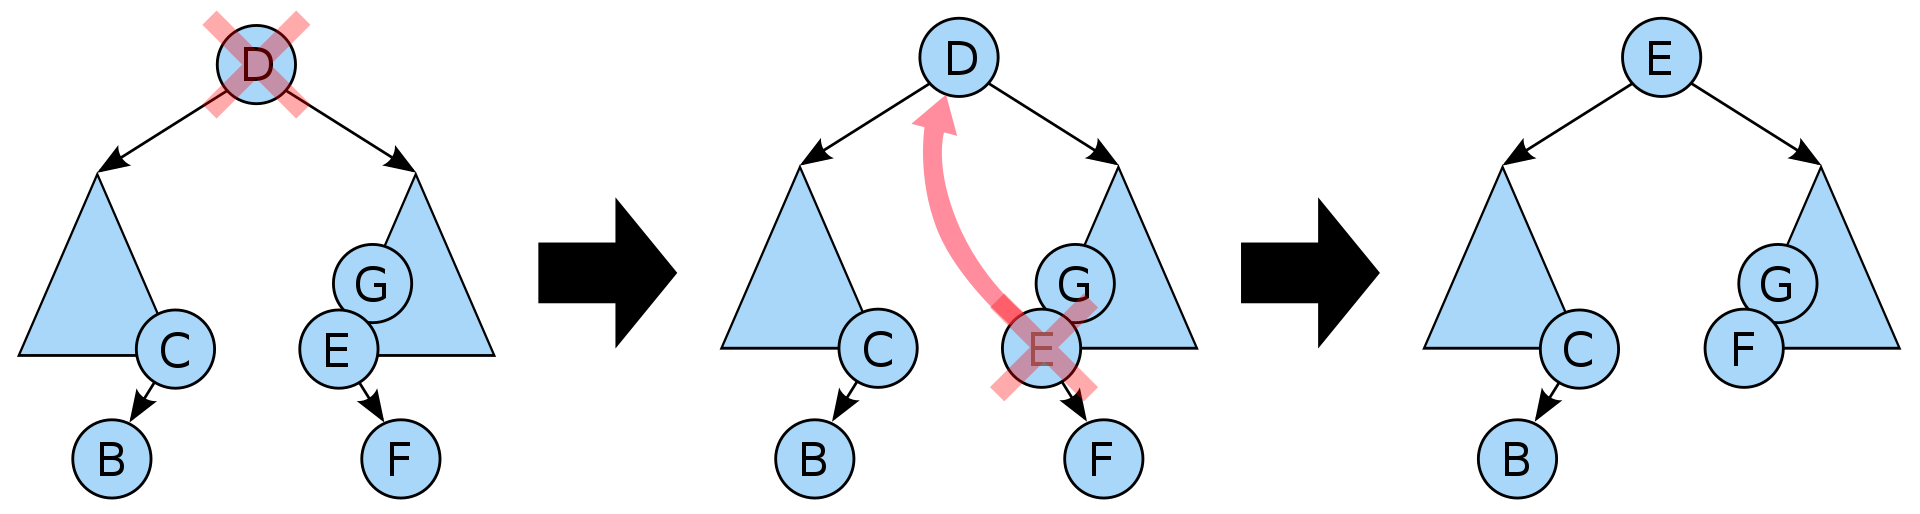
\includegraphics{binary_tree_delete.png}}
        \caption{Binárny vyhľadávací strom - mazanie uzlu}
    \end{figure}
    \end{center}
\end{frame}

%strana 9
\section{BVS - zložitosti operácií}
\begin{frame}{Zložitosť operácii nad BVS}
    \begin{figure}
    \begin{tabular}{||c c c||}\hline
         \bf{Algoritmus} & \bf{Priemerná zložitosť} & \bf{Najhoršia zložitosť} \\ [0.5ex] 
         \hline\hline
         Potrebný priestor & O(${n}$) & O(${n}$)\\ 
         \hline\hline
         Vyhľadávanie & O($\log{n}$) & O(${n}$)\\ 
         \hline\hline
         Vkladanie & O($\log{n}$) & O(${n}$)\\
         \hline\hline
         Mazanie & O($\log{n}$) & O(${n}$)\\
         \hline
    \end{tabular}
    \caption{Prehľad zložitosti operácii nad BVS}
    \end{figure}
\end{frame}

%strana 10
\section{Pseudokód operácii nad BVS}
\begin{frame}[fragile]{Pseudokód operácii nad BVS}
    \begin{itemize}
        \item{Vyhľadávanie v~BVS:}
    \end{itemize}
    \begin{lstlisting}
    def findval (node, lookfor):
    
        if (node is null):
            return null
            
        if (node.val is equal to lookfor):
            return node
            
        if (node.val is less than lookfor):
            return findval (node.right,lookfor)
            
        return findval (node.left,lookfor)
    \end{lstlisting}
\end{frame}

%strana 11
\begin{frame}[fragile]{Pseudokód operácii nad BVS}
    \begin{itemize}
        \item{Vkladanie - insert:}
    \end{itemize}
    \begin{lstlisting}
    def search(root,key):
    
        if (root is None) or (root.val == key):
            return root
     
        # Key is greater than root's key
        if (root.val < key):
            return search(root.right,key)
       
        # Key is smaller than root's key
        return search(root.left,key)
    \end{lstlisting}
\end{frame}

%strana 12
\begin{frame}{Zdroje}
    \begin{itemize}
        \item Wikipedia.org: Binary search tree\\
        \url{https://en.wikipedia.org/wiki/Binary_search_tree} 
        \item GeeksforGeeks.org: Binary Search Tree\\
        \url{https://www.geeksforgeeks.org/binary-search-tree-set-1-search-and-insertion} 
        \item StackOverflow.org: Pseudo-code for search in binary tree\\
        \url{https://stackoverflow.com/questions/4038328/pseudo-code-for-search-in-binary-tree} 
    \end{itemize}
\end{frame}
\end{document}